% CVPR 2022 Paper Template
% based on the CVPR template provided by Ming-Ming Cheng (https://github.com/MCG-NKU/CVPR_Template)
% modified and extended by Stefan Roth (stefan.roth@NOSPAMtu-darmstadt.de)

\documentclass[10pt,twocolumn,letterpaper]{article}

%%%%%%%%% PAPER TYPE  - PLEASE UPDATE FOR FINAL VERSION
%\usepackage[review]{cvpr}      % To produce the REVIEW version
\usepackage{cvpr}              % To produce the CAMERA-READY version
%\usepackage[pagenumbers]{cvpr} % To force page numbers, e.g. for an arXiv version

% Include other packages here, before hyperref.
\usepackage{graphicx}
\usepackage{amsmath}
\usepackage{amssymb}
\usepackage{booktabs}

\newcommand{\latex}{\LaTeX\xspace}
\newcommand{\tex}{\TeX\xspace}


% It is strongly recommended to use hyperref, especially for the review version.
% hyperref with option pagebackref eases the reviewers' job.
% Please disable hyperref *only* if you encounter grave issues, e.g. with the
% file validation for the camera-ready version.
%
% If you comment hyperref and then uncomment it, you should delete
% ReviewTempalte.aux before re-running LaTeX.
% (Or just hit 'q' on the first LaTeX run, let it finish, and you
%  should be clear).
\usepackage[pagebackref,breaklinks,colorlinks]{hyperref}


% Support for easy cross-referencing
\usepackage[capitalize]{cleveref}
\crefname{section}{Sec.}{Secs.}
\Crefname{section}{Section}{Sections}
\Crefname{table}{Table}{Tables}
\crefname{table}{Tab.}{Tabs.}


%%%%%%%%% PAPER ID  - PLEASE UPDATE
\def\cvprPaperID{*****} % *** Enter the CVPR Paper ID here
\def\confName{CVPR}
\def\confYear{2022}


\begin{document}

%%%%%%%%% TITLE - PLEASE UPDATE
\title{Detección de Rostros basada en la Red YOLOv3 Preentrenada}

\author{Alejandro Cárdenas Barranco\\
%Institution1\\
%Institution1 address\\
{\tt\small e.acarbar@go.ugr.es}
% For a paper whose authors are all at the same institution,
% omit the following lines up until the closing ``}''.
% Additional authors and addresses can be added with ``\and'',
% just like the second author.
% To save space, use either the email address or home page, not both
\and
Álvaro Rodríguez Gallardo\\
%Institution2\\
%First line of institution2 address\\
{\tt\small e.alvaro155w@go.ugr.es}
\and
Juan Manuel Rodríguez Gómez\\
{\tt\small e.juanmaarg6@go.ugr.es}
}
\maketitle

%%%%%%%%% ABSTRACT
\begin{abstract}

Este trabajo presenta un enfoque para la detección de rostros utilizando la red neuronal YOLOv3 preentrenada. A través de una implementación en Keras y la aplicación de técnicas de procesamiento de imágenes, 
hemos desarrollado un sistema capaz de detectar rostros en tiempo real con alta precisión. El proyecto abarca desde la configuración inicial del entorno de desarrollo hasta la evaluación práctica del modelo en un 
conjunto de imágenes de prueba. Los resultados destacan la eficiencia de YOLOv3 en la detección de rostros, demostrando su viabilidad para aplicaciones en tiempo real. Las contribuciones de este trabajo incluyen 
la adaptación del modelo YOLOv3 para la detección específica de rostros y la optimización de su rendimiento en términos de velocidad y precisión. Todos los archivos que han sido necesarios, además de un Jupyter Notebook
donde se ha desarrollado todo el código y se han obtenido los resultados correspondiente, se encuentran en este \href{https://drive.google.com/drive/folders/1dB7OtOwB2__0FQpF2SjowMTJx9Cuxit0?usp=drive_link} {enlace}.

   
\end{abstract}

%%%%%%%%% BODY TEXT
\section{Introducción}
\label{sec:intro}

Este proyecto se centra en la resolución de un desafío significativo en el campo de visión por computador: la \textbf{detección eficaz y precisa de rostros en imágenes}. La motivación detrás de este trabajo surge de la creciente
relevancia de la identificación y análisis de rostros en diversas aplicaciones, desde la seguridad hasta las interacciones sociales en plataformas digitales. La detección de rostros no solo es crucial para la identificación de 
individuos, sino también para el análisis de emociones y gestos, lo cual tiene implicaciones en sectores como el marketing, la seguridad pública y la interacción humano-computadora.

Para abordar este problema, hemos optado por implementar y optimizar la red neuronal \textbf{YOLOv3}, conocida por su rapidez y precisión en la detección de objetos. El objetivo concreto del proyecto es adaptar YOLOv3 para la 
detección específica de rostros, asegurando que el modelo funcione eficientemente. Esta adaptación implica no solo el entrenamiento y ajuste del modelo con un conjunto de datos adecuado, sino también la evaluación de su 
rendimiento en términos de velocidad y precisión, factores críticos para aplicaciones en tiempo real.

En resumen, este proyecto busca desarrollar una solución robusta y confiable para la detección de rostros, contribuyendo así al avance en el campo de visión por computador y abriendo puertas a nuevas aplicaciones y mejoras 
en sistemas existentes.

\section{Antecedentes}

Para comprender el trabajo desarrollado en este proyecto, es esencial familiarizarse con algunos conceptos clave en el campo de visión por computador y el aprendizaje profundo. Primero, la \textbf{visión por computador} es una disciplina 
científica que se enfoca en cómo las computadoras pueden adquirir, procesar, analizar y comprender las imágenes digitales. Dentro de esta área, la detección de objetos es una de las tareas más desafiantes y útiles, que implica identificar 
y localizar objetos dentro de una imagen.

El \textbf{aprendizaje profundo}, una rama del aprendizaje automático, ha revolucionado este campo, especialmente a través de las redes neuronales convolucionales (CNNs). Estas redes son particularmente efectivas para tareas de procesamiento de 
imágenes debido a su capacidad para aprender jerarquías de características visuales.

En el núcleo de nuestro proyecto se encuentra \textbf{YOLOv3 (You Only Look Once versión 3)}, una red neuronal con arquitectura completamente convolucional dirigida a detección de objetos que destaca por su velocidad y precisión. YOLOv3 es una CNN que divide la imagen en una cuadrícula y predice cuadros delimitadores 
y probabilidades de clases para cada celda de la cuadrícula simultáneamente, lo que le permite detectar objetos en una sola evaluación de la red, a diferencia de otros modelos que requieren varias pasadas. Este enfoque hace que YOLOv3 sea excepcionalmente rápido 
y adecuado para aplicaciones en tiempo real, un aspecto crucial para la detección de rostros. YOLOv3 realiza detección en 3 escalas distintas, de manera que devuelve un tensor3D para cada escala del mismo tamaño que la escala en la que está detectando, codificando la información de cada celda: las coordenadas de la caja, la puntuación de si es un objeto y puntuación de cada clase. Además, en cada escala se predicen 3 cajas a partir de la desviación que tengan con otras de tamaño prefijado (\textit{anchor boxes}).  En \hyperref[fig:fig1]{Figure 1} se puede observar la arquitectura de esta red. Esta arquitectura se divide principalmente en dos partes: Darknet-53 (es el extractor de características a distintas escalas) y Feature Pyramid Network (se encarga de detectar en 3 escalas distintas, pequeña, mediana y grande, resultantes de dividir las dimensiones de la imagen de entrada entre 32, 16 y 8 respectivamente.

\begin{figure*}[htbp]
\centering
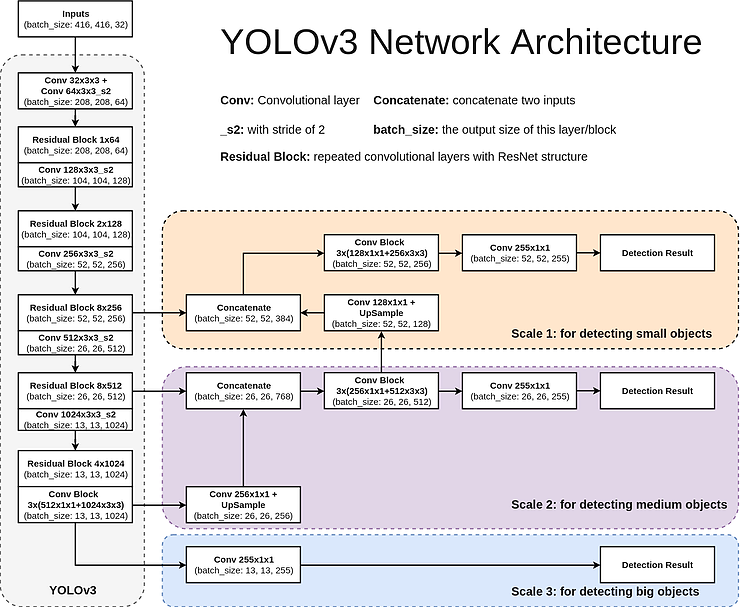
\includegraphics[width=\textwidth, height=10cm, keepaspectratio]{3.png}
\caption{Arquitectura de YOLOv3. Imagen extraída de \href{https://soprasteriaanalytics.se/2019/04/25/understanding-object-detection-using-yolo-and-training-for-new-objects-part-1/} {Sopra Steria Analytics}.}
\label{fig:fig1}
\end{figure*}

\section{Trabajos Relacionados}

El campo de la detección de objetos y, en particular, la detección de rostros, ha sido objeto de numerosos estudios y avances significativos en los últimos años. Un trabajo fundamental en este campo es el conjunto de datos \textbf{Microsoft COCO (Common Objects in Context)}
presentado por Lin et al. \cite{lin2015microsoft}. Este conjunto de datos ha sido ampliamente utilizado para entrenar y evaluar modelos de detección de objetos, incluyendo rostros, debido a su diversidad y amplitud.

En el ámbito específico de los modelos de detección de objetos, \textbf{YOLOv3}, descrito por Redmon y Farhadi \cite{redmon2018yolov3}, representa un hito importante. Este modelo es reconocido por su velocidad y precisión, y ha establecido un nuevo estándar en la detección de objetos en tiempo 
real. La arquitectura de YOLOv3 y su enfoque incremental ha influido en numerosos proyectos y aplicaciones.

Por último, la investigación de Yang et al. \cite{yang2016wider} en el benchmark \textbf{WIDER FACE} ha proporcionado una base importante para la detección de rostros. Este benchmark ofrece un conjunto de datos extenso y variado, específicamente diseñado para evaluar el rendimiento de los 
algoritmos de detección de rostros en diferentes escenarios.

Estos trabajos han sentado las bases y continúan influenciando el desarrollo de técnicas avanzadas en la detección de rostros, proporcionando tanto datos de calidad como metodologías innovadoras para la evaluación de modelos.

\section{Métodos}
\label{sec:metodos}

Nuestro enfoque para la detección de rostros implicó el desarrollo y evaluación de varios modelos:

\begin{itemize}
    \item \textbf{Modelo Base}: Comenzamos con un modelo base, utilizando los pesos preentrenados en COCO y añadiendo una capa de detección en cada escala. Este modelo sirve como referencia para comparar mejoras posteriores.
    \item \textbf{Modelo 1 - Entrenamiento Completo}: Se realizó el entrenamiento completo del modelo, partiendo de los pesos preentrenados en COCO y empleando técnicas de aumento de datos. Se experimentó con dos tamaños de entrada: 416 x 416 y 1024 x 1024, para evaluar el impacto del tamaño de entrada en la precisión del modelo.
    \item \textbf{Modelo 2 - Fine-tuning en los Bloques de Detección}: Esta fase implicó realizar fine-tuning específicamente en los bloques de detección de la red. Este proceso de fine-tuning permitió mejorar aún más la precisión del modelo en la detección de rostros,
											       ajustando el modelo a las características específicas de los datos de rostros utilizados.
    \item \textbf{Modelo 3 - Fine-tuning en el Extractor de Características}: El último modelo probado incluyó el congelamiento del extractor de características (las primeras 74 capas de la red - las 53 capas de Darknet-53 más 21 capas adicionales capas convolucionales adicionales que están configuradas para refinar o mejorar las características extraídas por el Darknet-53). Esta estrategia se centró en afinar las capas restantes para mejorar la detección.
\end{itemize}

Cada modelo fue evaluado rigurosamente, siendo cada una de estas etapas cruciales para alcanzar el alto nivel de precisión y eficiencia requerido para la detección de rostros en, lo que demuestra la meticulosidad y la profundidad del enfoque metodológico adoptado en este proyecto.

Cabe destacar el uso de diferentes \textbf{archivos de configuración JSON} que definen los entornos (valores de los diferentes parámetros, directorios, etc.) para los diferentes modelos.

\section{Experimentos}

\textbf{Datos}. El proyecto empleó dos datasets clave: \textbf{COCO} y \textbf{WIDER FACE}. El dataset COCO proporcionó una base amplia para el entrenamiento inicial con sus múltiples categorías y objetos. Por otro lado, el dataset WIDER FACE, especializado en rostros con diversas condiciones y contextos, permitió afinar el modelo específicamente para la detección de rostros. En las \hyperref[subsec:datasets]{Secciones 5.1 y 5.2} de este artículo se incluye una explicación más detallada de cada uno de estos conjuntos de datos. \\



\textbf{Protocolo de Validación Experimental}. Se han descargado los \textbf{pesos preentrenados de la red en el dataset COCO}. Estos pesos se corresponden a todas las capas convolucionales de YOLOv3, sin contar las capas de detección que dependen del dataset concreto que utilicemos. También se
descargado el \textbf{dataset WIDER FACE} (el cual ya viene dividido en conjunto de entrenamiento, conjunto de validación y conjunto test). Tras ello, fue necesario \textbf{generar las \textit{anchor boxes} para nuestro dataset WIDER FACE}. Ya dijimos que la red YOLOv3 predice \textit{offsets} respecto a estos valores predeterminados, por lo que si queremos entrenar la red con imágenes de nuestro nuevo conjunto WIDER FACE debemos proporcionar estas cajas prefijadas. Para ello, utilizamos un fichero con el código correspondiente que simplemente aplica el algoritmo de K-medias en el conjunto de entrenamiento para predecir 3 anchor boxes en cada escala, dadas en función del alto y del ancho. El resultado fue el siguiente:
$$[[2,4,4,8,7,14],$$
$$[12,23,20,36,35,56],$$
$$[56,95,101,149,177,234]].$$
Se ha hecho uso de una \href{https://github.com/experiencor/keras-yolo3}{implementación en Keras de la red YOLOv3}, la cual se tuvo que adaptar a Tensorflow 2. Esta implementación, trabaja con las \textbf{anotaciones de \textit{ground truth} en formato VOC}, por lo que tuvimos que convertirlas utilizando el código almacenado en un fichero.
Tras estas consideraciones previas al uso de la red, comentamos los principales aspectos de entrenamiento de la red:
\begin{itemize}
    \item \textbf{Data Augmentation}: Consideramos realizar un aumento de imágenes para obtener una mayor precisión en el conjunto de validación. Mediante dos parámetros de los archivos de configuración que disponemos podemos establecer los tamaños mínimo y máximo de las imágenes, que deberán ser siempre múltiplos de 32. Por limitaciones en el entorno utilizado (Google Colab) rara vez podremos superar tamaños de 512 × 512 para entrenar. A la hora de entrenar, las imágenes se redimensionan automáticamente cada 10 batches a algún tamaño comprendido entre el mínimo y el máximo que sea múltiplo de 32. También aplicamos transformaciones aleatorias de escala y recorte.
    \item \textbf{Tamaño del Batch}: Debido a las limitaciones en cuanto a la memoria disponible en el entorno utilizado, nos hemos visto obligados a utilizar un batch size de 4 para las imágenes de entrenamiento en todo momento.
    \item \textbf{Optimizador y Learning Rate}: Empleamos el optimizador Adam para compilar cada modelo. Comenzamos a entrenar los modelos con un learning rate de 0.001, que es el valor por defecto de este optimizador. Disponemos de un callback, que establece un learning rate 10 veces menor cada vez que llevemos dos épocas sin mejorar la función de pérdida. De esta forma conseguimos acelerar la convergencia en las épocas iniciales y ajustar gradualmente los pesos conforme avanzamos en el entrenamiento.
    \item \textbf{Épocas de "Calentamiento"}: Mediante un parámetro de los archivos de configuración, especificamos un número de épocas iniciales en las cuales las cajas predichas por el modelo deben coincidir en tamaño con los \textit{anchors} especificados. Lo fijamos a 3, y esto solo se aplica en las primeras épocas del entrenamiento.
    \item \textbf{Umbral de Predicción}: Internamente la red utiliza el un parámetro en los archivos de configuración para decidir qué hacer con una predicción. Si el solapamiento entre la caja predicha y el valor de \textit{ground truth} es mayor que dicho umbral, dicha predicción no contribuye al error. En otro caso, sí contribuye. Si este umbral es demasiado alto, casi todas las predicciones participarán en el cálculo del error, lo que puede causar overfitting. Por el contrario, si este valor es demasiado bajo perderemos demasiadas contribuciones al error y podríamos causar underfitting. Ponemos por defecto un valor de 0.5 para dicho umbral.
También se dispone de un parámetros que indica un umbral a partir del cual se considera que un objeto detectado es realmente un objeto (el resto se descartan). Se tiene otro parámetro que controla el umbral de la supresión de no-máximos realizada para eliminar detecciones solapadas.
    \item \textbf{Cálculo de la Función de Error}: También se dispone de cuatro parámetros en los archivos de configuración podemos fijar la escala en la que afecta cada parte al error total. El primero se refiere al error dado al predecir que algo es un objeto cuando en realidad no lo era, y el segundo a la acción contraria. El tercero controla el error en la predicción de las cajas frente a los valores reales, y el cuarto el error en la predicción de clase. Los valores por defecto son 5, 1, 1 y 1, respectivamente.
    \item \textbf{Otros callbacks}: Disponemos de un callback que va guardando un modelo con los mejores pesos obtenidos hasta el momento, de forma que podemos reanudar el entrenamiento por donde nos quedásemos. También tenemos un callback para detener el entrenamiento si no disminuye el error en 7 épocas (Early Stopping).\\
\end{itemize}

\begin{table*}[htb]
\centering
\begin{tabular}{c|c|c|c|c}
\textbf{Modelo}		& \textbf{Épocas de entrenamiento} & \textbf{Tamaño de entrada} & \textbf{\textit{mAP@[.5:.95]}} & \textbf{\textit{mAP@0.5}} \\
\hline
Modelo Base              & 10                              		     & 416 x 416                   	 & 0.025                     	  	  & 0.083          		 	    \\
Modelo 1-416           	& 16                              		     & 416 x 416                   	 & 0.257                     	  	  & 0.468           	 	    \\
Modelo 1-1024           & 15                              		     & 1024 x 1024                 	 & 0.376                   		  	  & 0.666             	 	    \\
Modelo 2        		& 20                               		     & 1024 x 1024                	 & \textbf{0.405}                 	  & \textbf{0.726}       	    \\
Modelo 3       		& 25                              		     & 1024 x 1024                       & 0.392                  		  	  & 0.708           	 	    \\
\end{tabular}
\caption{Resultados de la evaluación de los modelos.}
\label{tabla:resultados_evaluacion}
\end{table*}

\textbf{Métricas}. Para evaluar los modelos usaremos las dos siguientes métricas mAP (mean Average Precision):
\begin{itemize}
    \item \textbf{\textit{mAP@0.5}}: Esta métrica calcula el mAP con un umbral de IoU (Intersection over Union) de 0.5.
    \item \textbf{\textit{mAP@[.5:.95]}}: Esta métrica calcula la media de los mAP para varios umbrales de IoU, desde 0.5 hasta 0.95, en pasos de 0.05. \\
\end{itemize}

\textbf{Experimentos}. Tras definir las correspondientes funciones para entrenar y evaluar los diferentes modelos usando los parámetros del correspondiente archivo de configuración JSON, se han generado los modelos descritos en la \hyperref[sec:metodos]{Sección 4} de este artículo:

\begin{itemize}
    \item \textbf{Modelo Base}: Comenzamos con un modelo base, utilizando los pesos preentrenados de COCO y añadiendo una capa de detección en cada escala. Utilizamos los parámetros por defecto (se pueden ver en el archivo de configuración JSON correspondiente) y elegimos un tamaño de entrada de 416 × 416. Lo entrenamos durante 10 épocas (más las 3 épocas de "calentamiento"), congelando todas las capas excepto las 3 añadidas. Cada época ha tardado unos 360 segundos (6 minutos) aproximadamente (excepto la primera época de "calentamiento", la cual siempre tarda más, tardando en este caso 2400 segundos aproximadamente, es decir, 40 minutos). El loss fue disminuyendo hasta estancarse en aproximadamente 13.1. 

    \item \textbf{Modelo 1 - Entrenamiento Completo}: Se realizó el entrenamiento completo del modelo, partiendo de los pesos de COCO y empleando técnicas de aumento de datos. Se experimentó con dos tamaños de entrada: 416 x 416 y 1024 x 1024, para evaluar el impacto del tamaño de entrada en la precisión del modelo.
									      
Para un tamaño de entrada de 416 x 416, este modelo iba a ser entrenado durante unas 20 épocas (más las 3 épocas de "calentamiento"), pero desde la época 10 el loss se estancó en 20.7 durante las próximas 7 épocas, por lo que se produjo Early Stopping. Cada época ha 									      tardado unos 600 segundos (10 minutos) aproximadamente (excepto la primera época de "calentamiento", la cual siempre tarda más, tardando en este caso 4200 segundos aproximadamente, es decir, 1 hora y 10 minutos). Intentamos reiniciar el entrenamiento partiendo de un learning rate más elevado para escapar del óptimo local, pero este enfoque no surtió efecto.

Para un tamaño de entrada de 1024 x 1024, este modelo también iba a ser entrenado durante unas 20 épocas (más las 3 épocas de "calentamiento"), pero debido a falta de GPU en el entorno utilizado (Google Colab), el entrenamiento se detuvo en la época 16. Cada época ha tardado unos 780 segundos (13 minutos) aproximadamente (excepto la primera época de "calentamiento", la cual siempre tarda más, tardando en este caso 3960 segundos aproximadamente, es decir, 1 hora y 6 minutos). Nótese el incremento en el tiempo de ejecución de cada época de este modelo con respecto al anterior (esto es debido al aumento del tamaño de entrada). El loss fue disminuyendo hasta estancarse en aproximadamente 22.8.

    \item \textbf{Modelo 2 - Fine-tuning en los Bloques de Detección}: Esta fase implicó realizar fine-tuning específicamente en los bloques de detección de la red. Establecimos el umbral de predicción a 0.7 y aumentamos al doble la contribución al error de las diferencias entre las cajas predichas y las verdaderas. Hacemos todo esto para intentar mejorar la precisión. Partimos de los pesos de COCO y dividimos el entrenamiento en dos partes.

La primera parte del entrenamiento consiste en congelar toda la red excepto las 4 últimas capas de cada escala. Entrenamos el modelo durante 10 épocas (más las 3 épocas de calentamiento). Cada época ha tardado unos 360 segundos (6 minutos) aproximadamente (excepto la primera época de "calentamiento", la cual siempre tarda más, tardando en este caso 2100 segundos, es decir, 35 minutos). El loss fue disminuyendo hasta estancarse en aproximadamente 22.8.

Para la segunda parte del entrenamiento, se descongelaron todas las capas. Este modelo iba a ser entrenado durante unas 20 épocas (ahora no se tienen épocas de "calentamiento"), pero debido a falta de GPU en el entorno utilizado (Google Colab), el entrenamiento se detuvo en la época 11. Cada época ha tardado unos 660 segundos (11 minutos) aproximadamente (excepto la primera época, la cual siempre tarda más, tardando en este caso 3600 segundos aproximadamente, es decir, 1 hora). Esta vez se parte de un learning rate inicial de $10^{-4}$ . El loss fue disminuyendo hasta estancarse en aproximadamente 4.5.

    \item \textbf{Modelo 3 - Fine-tuning en el Extractor de Características}: El último modelo probado incluyó el congelamiento del extractor de características (las primeras 74 capas de la red - las 53 capas de Darknet-53 más 21 capas adicionales capas convolucionales adicionales que están configuradas para refinar o mejorar las características extraídas por el Darknet-53). Esta estrategia se centró en afinar las capas restantes para mejorar la detección.

En la primera etapa entrenamos 10 épocas (más las 3 épocas de "calentamiento") partiendo de un learning rate de 0.001. Cada época ha tardado unos 720 segundos (12 minutos) aproximadamente (excepto la primera época de "calentamiento", la cual siempre tarda más, tardando en este caso 2700 segundos aproximadamente, es decir, 45 minutos). El loss fue disminuyendo hasta estancarse en aproximadamente 14.3.

Para la segunda etapa del entrenamiento, entrenamos el modelo completo (se descongelaron todas las capas) durante 15 épocas. Cada época ha tardado unos 660 segundos (11 minutos) aproximadamente (excepto la primera época, la cual siempre tarda más, tardando en este caso 3600 segundos aproximadamente, es decir, 1 hora). El loss fue disminuyendo hasta estancarse en aproximadamente 5.8.
\end{itemize}

\textbf{Resultados y Discusión}. Tras evaluar los modelos descritos anteriormente, se han obtenido los resultados mostrados en \hyperref[tabla:resultados_evaluacion]{Table 1}. La progresión en las métricas de los modelos entrenados muestra una mejora clara en la detección de rostros a medida que se incrementa la complejidad del entrenamiento y el ajuste del modelo. El Modelo Base establece una línea de base con \textit{mAP@[.5:.95]} y \textit{mAP@0.5} relativamente bajos, lo cual mejora significativamente con el Modelo 1, especialmente al aumentar el tamaño de entrada a 1024 x 1024, indicando la \textbf{relevancia de la resolución de entrada en la precisión de la detección}.
El Modelo 2, que incorpora \textbf{fine-tuning}, alcanza las puntuaciones más altas en ambas métricas, destacando la \textbf{efectividad} de esta técnica para optimizar la red para una tarea específica como la detección de rostros. Sin embargo, el Modelo 3, a pesar de adoptar una estrategia de congelar el extractor de características, no supera al Modelo 2, sugiriendo que el fine-tuning de todo el modelo es más beneficioso para este conjunto de datos y tarea específica. Esto implica que \textbf{la capacidad de adaptarse a características de bajo nivel es importante para la detección de rostros y debe mantenerse flexible durante el entrenamiento}. \\

\textbf{Ejemplos de Detección}. En \hyperref[fig:fig2]{Figure 2} se observan un par ejemplos de caras detectadas con el Modelo 2 (que es con el que se han obtenido mejores resultados en las métricas utilizadas). En general, se ha observado es que el modelo consigue detectar caras muy bien cuando están bien separadas, e incluso las caras pequeñas o de perfil consigue detectarlas. Cuando hay muchas caras juntas y superpuestas (por ejemplo un grupo de personas en una foto tomada de lejos) a veces no detecta correctamente todas las caras. Sin embargo, en muchas fotos consigue detectar la mayoría con gran precisión.

\subsection{Dataset COCO}
\label{subsec:datasets}

Se ha partido de los pesos de YOLOv3 después de ser entrenada en el dataset \textbf{COCO (Common Objects in COntext)}. COCO fue desarrollado por Microsoft en colaboración con académicos de varias universidades. Se lanzó por primera vez en 2014 y desde entonces ha sido una referencia estándar 
en la comunidad de visión por computador.

Este conjunto de datos contiene más de \textbf{200,000 imágenes etiquetadas}, con \textbf{más de un millón de objetos etiquetados en 80 categorías diferentes} como personas, animales, vehículos y objetos cotidianos. Las imágenes son de la vida real y proporcionan una amplia gama de contextos y escenarios.
COCO es particularmente valorado por su enfoque en la contextualización de los objetos, proporcionando no solo las etiquetas de los objetos, sino también información sobre su contexto en las escenas. Este enfoque lo hace ideal para entrenar y evaluar modelos de detección de objetos como YOLOv3.

Para la tarea de reconocer caras no es necesaria toda la información de los distintos objetos reconocidos en COCO, pero si hemos el reconocimiento de personas como base para nuestro detector de rostros.

\begin{figure}[h]
	\begin{subfigure}{0.5\textwidth}
		\centering
		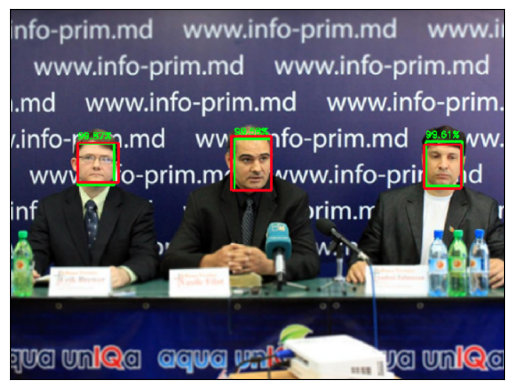
\includegraphics[width=0.9\linewidth, height=4.9cm, keepaspectratio]{1.png}
		\caption{Pocos rostros y separados entre ellos.}
		\label{fig:img1}
	\end{subfigure}
	\begin{subfigure}{0.5\textwidth}
		\centering
		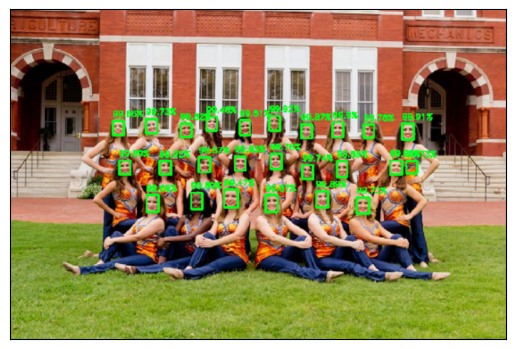
\includegraphics[width=0.9\linewidth, height=5cm, keepaspectratio]{2.png}
		\caption{Muchos rostros y próximos entre ellos.}
		\label{fig:img2}
	\end{subfigure}
\captionsetup{justification=centering}
\caption{Ejemplos de detección de rostros en imágenes (en verde la caja predicha por la red y en rojo el valor real de \textit{ground truth}).}
\label{fig:fig2}
\end{figure}

\subsection{Dataset WIDER FACE}

Se ha usado el dataset \textbf{WIDER FACE} para entrenar y evaluar los diferentes modelos. Este dataset es público (al igual que COCO) y está \textbf{específicamente diseñado para la detección de rostros en imágenes}. Proporciona un gran conjunto de imágenes con una amplia gama de condiciones y escenarios, lo que
 lo hace muy útil para entrenar y evaluar algoritmos de detección de rostros.

El conjunto de datos contiene \textbf{más de 32,000 imágenes en total y 393,703 caras etiquetadas y anotadas con cuadros delimitadores}, lo que facilita su uso en tareas de detección. Esto hace que sea uno de los conjuntos de datos más grandes y
 diversos para la detección de rostros. Las imágenes incluyen una gran variedad de escenarios, desde rostros en primer plano hasta rostros en multitudes y bajo diversas condiciones de iluminación.

Para la evaluación se proporcionan 16,151 imágenes (conjunto de test) de distribución similar al de entrenamiento pero con imágenes nuevas para comprobar el buen funcionamiento de la red. Sin embargo, no se liberan los valores de \textit{ground truth} para este conjunto y las competiciones asociadas y los servidores de evaluación están inactivos en este momento. Por lo tanto, se ha usado el conjunto de validación para evaluar los resultados, el cual contiene 3.230 imágenes.

\section{Conclusiones}

\textbf{Este proyecto ha demostrado exitosamente la capacidad de adaptar la red YOLOv3, preentrenada en COCO, para la detección eficaz de rostros, logrando una precisión notable sin conocimiento previo específico sobre objetos tipo rostro}. A pesar de las limitaciones en la métrica COCO, que prioriza la precisión de los \textit{bounding boxes} sobre la clasificación, YOLOv3 ha mostrado un desempeño comparable a las mejores redes en la métrica \textit{mAP@0.5}.

Se identifican oportunidades para \textbf{futuras investigaciones y mejoras}, como experimentar con diferentes optimizadores o ajustar aún más la red congelando bloques específicos. Además, aunque YOLOv3 es eficiente en detección en tiempo real, existen alternativas como Faster R-CNN o RetinaNet que podrían ofrecer mayor precisión, sacrificando la velocidad. Para aplicaciones prácticas, la elección entre YOLOv3 y otras redes dependerá de si se prioriza la velocidad de detección o la precisión.

Este estudio sienta las bases para exploraciones futuras en la detección de rostros, con un énfasis en \textbf{equilibrar precisión y eficiencia según las necesidades de la aplicación}. \\ \\ \\

%%%%%%%%% REFERENCIAS
{\small
\bibliographystyle{ieee_fullname}
\bibliography{egbib}
}

\end{document}
